\begin{document}

\section{Kursfolge-Indikator}
Die Idee zu diesem Indikator entstand während der Untersuchungen zu den Kursverläufen. Dabei wurde untersucht, ob die verschiedenen Kryptowährungen anderen Kryptowährungen folgen. Folgt ein Kurs einem zweiten Kurs zum Beispiel mit einem Tag Versatz, so kann eine Kauf-, Halte- bzw. Verkaufsempfehlung auf Basis des Kursverlaufes des zweiten Kurses gegeben werden.

\subsection{Umsetzung}
Zur Umsetzung des Indikators wird auf dem Ergebnisdatensatz eines Indikators gearbeitet. Auf Basis dieser Daten werden verschiedenen Berechnungen durchgeführt. Im Anschluss daran werden die Ergebnisse zusammengefasst und als .csv-Dateien exportiert. 

\subsubsection{Datensatz}
Der verwendete Datensatz besteht aus CSV-Dateien, welche je Tag Kursdaten von verschiedenen Kryptowährungen enthalten. Die enthaltenen Kursdaten sind der Kursname, das Datum, der Eröffnungskurs, der Schlusskurs, Tageshöchststand, Tagestiefstwert, das gehandelte Volumen sowie die Empfehlung des Indikators. Der Datensatz reicht von April 2013 bis Januar 2020.

\subsubsection{Analyse}
Die Analyse der Kursverläufe erfolgt dabei jeweils auf Basis der Empfehlungen eines Indikators. Die Indikatoren in dieser Arbeit geben ihre Empfehlungen in jeweils vier Stufen in den drei Klassen Kaufen, Halten und Verkaufen ab.
\begin{description}
\item[Kaufen] K0, K1, K2, K3
\item[Halten] H0, H1, H2, H3
\item[Verkaufen] V0, V1, V2, V3
\end{description}

Die Empfehlung V0 entspricht dabei einer schwachen Empfehlung den Kurs zu verkaufen, V3 dagegen einer starken Verkaufsempfehlung. Gleiches gilt respektive für die Klassen Halten und Kaufen.

Es werden die Empfehlung eines Kurses am Tag x mit der Empfehlung eines anderen Kurses am Tag x-1 (ein Tag vorher) verglichen. Je nach Übereinstimmung der beiden Empfehlungen, werden Punkte nach dem in Abbildung \ref{fig:punktesystem} gezeigten Schema vergeben.

\begin{figure}[h]
\centering
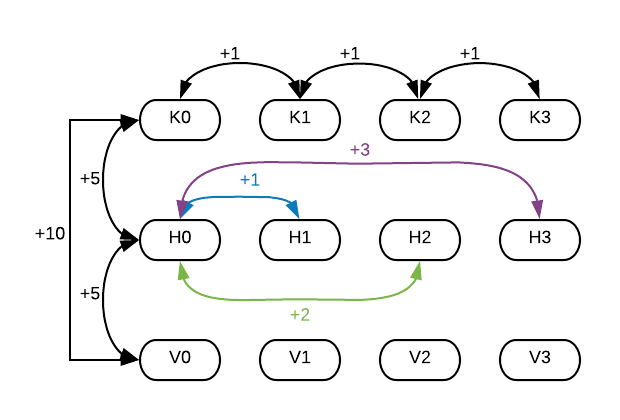
\includegraphics[width=\linewidth]{kursvergleich/punktesystem}
\caption{Punktesystem für die Bewertung der Übereinstimmung von zwei Kursen}
\label{fig:punktesystem}
\end{figure}

Sind beide Empfehlungen identisch (z.B. beide H3) werden 0 Punkte vergeben. Befinden sich beide Empfehlungen in derselben Klasse, zum Beispiel KursA H0 und KursV H2, so wird der Abstand zwischen den beiden als Punktzahl vergeben (in dem Beispiel sind dies 2 Punkte). Sind die Empfehlungen in unterschiedlichen, jedoch direkt nebeneinander liegenden Klassen, werden 5 Punkte zusätzlich zum Abstand addiert. Ein Beispiel hierfür wäre KursA H1 und KursV K0. Diese Konstellation würde mit 6 Punkten bewertet. Im letzten Fall hat ein Kurs eine Kaufempfehlung während der Vergleichskurs eine Verkaufsempfehlung hat. In diesem Fall werden 10 Punkte zusätzlich zum Abstand addiert (KursA V1, KursV K2 -> 13 Punkte).

\subsubsection{Auswertung}
Ist die Bewertung der Empfehlung eines Kurses zu den Empfehlungen der anderen Kurse abgeschlossen, wird der Durchschnitt der vergangenen drei Tage ermittelt. Hierdurch wird der Einfluss von Zufallstreffern (beide Kurse haben gleiche Empfehlung) minimiert.

Aus diesem Durchschnitt wird anschließend der Kurs mit der minimalen Punktezahl ermittelt. Dieser stellt den potentiellen Vergleichskurs oder ''Führungskurs'' dar, d.h. KursA folgt diesem. Es kann jedoch vorkommen, dass es mehrere Kurse mit der gleichen minimalen Punktezahl gibt. In diesem Fall wird der Kurs ausgewählt, welcher an dem jeweiligen Tag das größte Handelsvolumen aufweist, da diese potentiell mehr Einfluss am Markt haben. Abschließend wird geprüft, ob die Bewertung des Führungskurs kleiner als 5 ist, da Werte größer als 5 auf Empfehlungen in zwei verschiedenen Klassen deuten und sich der Verlauf der Kurse deshalb nicht ähnelt. Sollte aufgrund dieses Kriteriums kein Vergleichskurs mehr übrig bleiben wurde für den Ausgangskurs kein passender, vorlaufender Kurs gefunden.  

Der verbleibende Kurs ist der der Vergleichskurs dem der jeweilige Ausgangskurs folgt. Aus der Empfehlung des Vergleichskurses wird durch Vergleich mit der Empfehlung des Ausgangskurs eine neue Empfehlung abgeleitet. Stimmen die beiden Empfehlungen überein, wird das Signal verstärkt. Liefert der Ausgangskurs zum Beispiel ein schwaches Kaufsignal und der Vergleichskurs ein starkes, so wird als neue Empfehlung ebenfalls ein starkes Kaufsignal gesetzt. Liegen die Signale dagegen gegensätzlich, d.h. KursA bei V3 und KursV bei K2 wird eine Halteempfehlung ausgegeben.

Wird hingegen kein Vergleichskurs gefunden, kann auch keine Empfehlung abgegeben werden. Um den Wert NULL zu vermeiden und dadurch die Weiterverarbeitung einfacher zu gestalten, wird die originale Indikatorempfehlung aus den Basisdaten eingetragen.  

\subsubsection{Datenexport}
Die Ergebnisse aus der Analyse werden für die Weiterverarbeitung wieder in CSV-Dateien geschrieben und exportiert. Um die Weiterverarbeitung im Recommender-System zu vereinfachen, wird die gleiche Struktur wie beim Import der Daten verwendet. 

\subsection{Bewertung des Indikators}
Die Empfehlungen, mit welchen hier vorwiegend gearbeitet wird um die Kurse zu vergleichen, basieren auf Indikatorergebnissen bzw. -signalen. In Abhängigkeit von den verschiedenen Marktphasen (Bullen-, Bären- und Seitwärtsmarkt) kann die Qualität dieser Signale und damit die daraus abgeleiteten Empfehlungen stark variieren und teilweise vollkommen falsch liegen. Auf dieser Basis ist auch das Ergebnis diese Indikators mit Vorsicht zu betrachten, da sich die Fehler ergänzen aber auch aufheben können. 

\end{document}
